We have run two different versions of the model: one that is the same as \cite{li2018deep} in order to report on the original paper's reproducibility and another version that runs the newly proposed hierarchical version of this model. Firstly, we will discuss the replicated results of the original paper. Secondly, we will discuss the results of the hierarchical model.

\begin{figure}
    \centering
    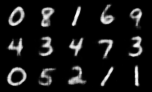
\includegraphics{img/normalprot1499.png}
    \caption{Original prototypes after 1500 epochs}
    \label{normalprots}
\end{figure}

After training our implementation of the original prototype model for 1500 epochs with 15 prototypes and a learning rate of 0.0001 as done by \cite{li2018deep} we achieved an accuracy of 98.8\%. This result affirms the fact that the results of the original paper are replicatable. Moreover, it shows that the addition of a prototype layer does not significantly reduce the accuracy that the model is able to achieve. 

The learned prototypes are represented with an encoded representation that can be decoded by running the prototypes through the trained decoder. This will return an image of the same size as the images in the training data. We passed the learned prototypes through our encoder, and the 15 prototypes that our implementation of the original prototype network produced are shown in Figure \ref{normalprots}. Just like in the original paper \cite{li2018deep}, the prototypes resemble authentic handwritten digits. Again, this confirms the fact that we can replicate the original paper, thereby producing meaningful and interpretable prototypes.

Subsequently, we extended the architecture in the original paper \cite{li2018deep} and we implemented and trained this hierarchical prototype model. After training the hierarchical prototype model for 1500 epochs, it achieved 98.6\% accuracy and 98.8\% accuracy for the superprototype classification network and the subprototype classification network respectively on the MNIST test set. These accuracies are very similar to the ones found in our implementation of the original prototype paper and the accuracy reported in \cite{li2018deep}, pointing to the fact that our hierarchical prototype model is equally as capable of making accurate predictions on the MNIST as the other two models are. 
\begin{figure}[ht]
    \centering
    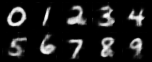
\includegraphics{img/prot1499.png}
    \caption{Superprototypes after 1500 epochs with weights set to negative identity.}
    \label{superprots}
\end{figure}

Next, by passing the learned superprototypes through the trained decoder, we can visualize the learned superprototypes as shown in Figure \ref{superprots}. The weight matrix connecting the 10 class superprototype layer to the 10 class softmax output layer can be fixed to the negative identity matrix. Fixing the weight matrix to the negative identity matrix ensures that we learn 10 prototypes that each resemble a distinct class within our data \cite{li2018deep}. For the MNIST data set, these classes are the digits 0-9. Because of the fixed weight matrix, the superprototypes shown in Figure \ref{superprots} each represent a different digit corresponding to our expectation. The learned superprototypes appear to be very crisp representations of handwritten digits, making the superprototypes interpretable.
\begin{figure}[ht]
    \centering
    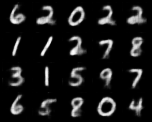
\includegraphics{img/subprot1499.png}
    \caption{20 subprototypes after 1500 epochs with learnable weights}
    \label{subprots}
\end{figure}

Simultaneous with training the superprototypes we train the subprototypes in our model. Again, we can visualize these subprototypes by passing their latent representations through the decoder and displaying the results as shown in Figure \ref{subprots}. The weight matrix connecting the 20 neuron subprototype layer to the 10 class output layer has learnable parameters. This allows our network to figure out for itself how many subclasses it learns for each class within the fixed number of subprototypes. As shown in Figure \ref{subprots} the model finds at least one subprototype per class. 

Consequently, some interesting subprototypes show up. The model finds 4 different visualisations of a 2. Apparently, it learns to model a number of different ways the two can be written, whether it is more straight or has a loop connecting the bottom part to the main diagonal. For the 1's, our model learns 3 different representations, mostly variations in how much they are tilted to the right. The variations in the 6's follow a similar pattern. Finally, some subprototypes represent mostly a specific class but can also be construed as trying to capture several digits at once and use it in their classification. For example, the 8 in the $3^{\text{rd}}$ column, $4^{\text{th}}$ row can also be seen as being a hybrid between an 8 and a 9. 
